\documentclass[14pt]{book}
\usepackage{graphicx}

\newenvironment{loggentry}[2]% date, heading
{\noindent\textbf{#2}\newline\{\marginnote{#1}\}\newline\\}{\vspace{1.0cm}}

\begin{document}
\begin{titlepage}
	\centering
	
\includegraphics[width=0.15\textwidth]{res/inf.png}\par\vspace{1cm}
	{\scshape\LARGE UFRGS - Instituto de Informatica \par}
	\vspace{1cm}
	{\scshape\Large Volunteer Project\par}
	\vspace{1.5cm}
	{\huge\bfseries Kelvinlets Video Deformation\par}
	\vspace{2cm}
	{\Large\itshape Guilherme Gomes Haetinger\par}
	\vfill
	supervised by\par
	Dr. Eduardo S. L. \textsc{Gastal}

	\vfill

% Bottom of the page
	{\large \today\par}
\end{titlepage}

\begin{figure}
	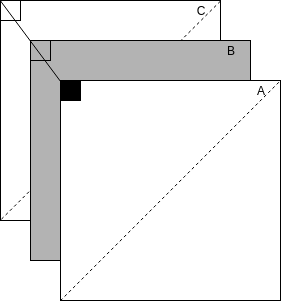
\includegraphics[width=\linewidth]{./res/interpolationExample.png}
	\caption{3D Interpolation with Prism projection}
	\label{fig:newInterp}
\end{figure}

\begin{loggentry}{28-05-2019}{New Idea for 3D Interpolation}
	Based on the idea of interpolating 3D Cuboids on video frames, I wonder: are there other (better) ideas for this instead of Interpolating the tetrahedrons inside the prisms? One hypothesis is a prism projection on the video frames [\ref{fig:newInterp}].	

	The idea of establishing Scan Conversion on the Frame mesh based solely on line interpolation between the preprocessed grids seems really faster than the tetrahedron approach. Whereas we would process every point inside a bounding box delimited by the corners of every tetrahedron inside a Cuboid (6 volumes), we now process one pixel related to 2 others, which colors will interpolate, and scan convert the remaining pixels of the frame with the produced ones, as we would do in the KelvinletsImageGL code. I like to call this new method 2 step interpolation.  
\end{loggentry}

\begin{loggentry}{30-05-2019}{Elaborating Implementation for 2 step Interpolation}
		Having in mind the Professor's advice to use a \textit{bin sort} alike algorithm, the main goal is to set which lines collide with each of the frames. We do that by assigning each vertex from the frame having 2 points: one in each deformed frame. Based on that, we can establish the color and position of the vertices. Now, considering the order that the vertices must be processed, we should run them by the time axis, i.e. Interpolate the same pixel position for each frame before moving to another position.    
\end{loggentry}

\begin{loggentry}{01-06-2019}{Project Structure}
	bla bla bla bla
\end{loggentry}

\end{document}
